\newcommand{\andop}{\operatorname{AND}}
\newcommand{\orop}{\operatorname{OR}}
\newcommand{\notop}{\operatorname{NOT}}

In this section we highlight the notion of a boolean expression as a function. Using this perspective it will be clear what it means for two expressions to be logically equivalent. 

\begin{tcolorbox}
A function will take a value (a number, an animal, anything) and output another value (a letter of the alphabet, the number of the animal's legs, anything). Later on we will learn a more rigorous definition than that described above.
\end{tcolorbox}

Then a boolean expression is really a function. Each variable takes in either true or false, at which point we can \textit{evaluate} the expression and we get some boolean value (either true or false). Consider the expression
\[(p \land q) \lor r.\]
Then we can feed in any combination of trues or falses. For example, if $p \equiv T$, $q \equiv F$, and $r \equiv T$, then the expression above will evaluate these values to 
\[(T \land F) \lor T \equiv F \lor T \equiv T,\] or true.

A \textbf{truth table} is then really just a way of recording the output values of this function. We summarize our findings here:
\begin{tcolorbox}
Two logical expressions are called \textbf{logically equivalent} if they have the same truth value given a set of truth values for each variable.

Equivalently, two logical expressions are logically equivalent if they have the same truth table.
\end{tcolorbox}

Let's consider the special case where our logical expression is $p \otimes q$ for a binary logical operator $\otimes$. This can be seen as a function of $p$ and $q$. So we might write it using notation like
\[O(p, q) = p \otimes q.\]
For instance, we might consider the expression $(p \land q) \lor r$ once again. Then we can view this expression in the notation
\[\orop(\andop(p, q), r).\]
This notation is also useful as it makes unambiguous how expressions are evaluated. This brings us to the topic of when expressions are ambiguously defined. For example, consider the expression $p \land q \lor r$. This is ambiguously defined. It could mean the following two expressions (when given in functional notation):
\begin{gather}
\orop(\andop(p, q),r) \\
\andop(p, \orop(q, r)).
\end{gather}
These expressions are not the same! So the expression being considered is called ``ambiguous''. This makes clear that when evaluating a logical expression it matters which part of the expression you evaluate first. However, there are some expressions where this does not matter. For example, the logical expression $p \land q \land r$ is unambiguous, because no matter if you take this expression to be $(p \land q) \land r$ or $p \land (q \land r)$, the resulting truth table remains the same. This pattern with repeated ands turns out to be unambiguous for any number of variables, but showing that this is true is somewhat difficult (and will be addressed as a topic in a later chapter).

In general, logical operators follow a certain pattern which lets us recursively evaluate them. Such evaluation lets modern computers (such as the one that this book was typeset) evaluate these expressions much like a computer would. For simplification we will assume that our logical expression consists of only boolean variables (like $p$, $q$, etc.), $\land$, $\lor$, and $\shortsim$ (and as we will see in a following section this actually will not lose any generality). Then any logical expression is of one of the following forms:

\begin{itemize}
	\item Some boolean variable $p$.
	\item $\andop(e_1, e_2)$, where $e_1$ and $e_2$ are logical expressions.
	\item $\orop(e_1, e_2)$, where $e_1$ and $e_2$ are logical expressions.
	\item $\notop(e)$, where $e$ is an expression.
\end{itemize}

Then we can proceed to evaluate the expressions, which are either one or two simpler logical expressions, or just a boolean variable which we evaluate to $T$ or $F$ depending on what evaluation we wanted to do.

In general computers, when interpreting a logical expression like
\[(p \land q) \lor r\]
will convert this expression into function notation as above, and then evaluate the expression once it has been converted using the rules above.
\begin{enumerate}
   \item Create truth tables for the following expressions.

\begin{itemize}
    \item $p \land (\sim p)$ (This formula is called \textit{unsatisfiable}. Why is this?)
    \item $p \land T$ (Here, $T$ represents true. Similarly, $F$ represents false).
    \item $p \land F$
    \item $p \lor T$ and $p \lor F$.
\end{itemize}


    \item Let's consider the logical expressions in problem 1 again. Figure out simpler expressions which are equivalent to these.
    \item Consider the following chunk of code. Here, \verb|var1|, \verb|var2| are boolean variables (ie, they are true or false).
\begin{verbatim}
    if (var1 && (var1 || var2)) { printf("She loves me!"); }
    else { printf("She loves me not..."); }
\end{verbatim}
Simplify the code.


    \item We have made it a point in this section that given a logical expression (or even an arithmetic expression), parentheses matter!

Build the truth tables for $(\sim a) \land b$ and $\sim (a \land b)$. Compare it to the viral facebook math problem below:

\begin{figure}[ht]
    \centering
    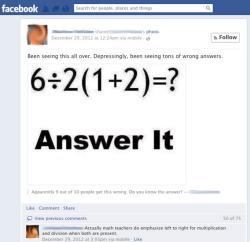
\includegraphics{Ch1/arithmetic.jpg}
    \caption{Viral Facebook Math Meme}
    \label{fig:arithmetic}
\end{figure}
    \item This problem mostly deals with the implies $(\implies)$ logical operator. The motivation behind this operator is that eventually we want to do \textbf{proofs}. That is, given a set of initial hypotheses, we want to make deductions and logically deduce that a conclusion is true. For example, eventually all of you will be able to prove, roughly stated:
\[(\text{$n$ is even}) \implies (\text{$n + 1$ is odd}).\]

Construct the truth tables for all the logical expressions below.
%I'll cover the first two bullets in class.
\begin{itemize}
    \item $p \implies (p \land q)$ and $p \implies (p \lor q)$.
    \item $(p \land q) \implies (p \lor q)$. This formula is an example of a \textit{tautology}.
    \item $(p \lor q) \implies (p \land q)$.
    \item $(p \implies q) \implies (p \iff q)$.
    \item $(p \iff q) \implies (p \implies q)$.
    \item $p \implies q \implies r$ and $p \implies r$.
\end{itemize}
    \item Convert the following expressions into functional notation. If the expression is ambiguous, then list all possible functions which the expression could represent. Use $\operatorname{NAND}$ for the $\uparrow$ operator and $\operatorname{NOT}$ for the $\shortsim$ operator. (For a unary operator, $\operatorname{NOT}$ takes how many variables?)

\begin{itemize}
	\item $(p \uparrow q) \lor (q \land p)$
	\item $\shortsim p \lor q$
	\item $p \lor q \uparrow r \land s$
\end{itemize}
    \item In this problem we will outline how one can write a computer program that can parse and evaluate logical expressions such as $\shortsim(T \lor F) \land (F \lor T)$. For the sake of simplicity, we may assume that any logical expression only consists of the standard and ($\land$), or ($\lor$), and not ($\shortsim$) operators.

\begin{enumerate}
	\item Scan the input string and form a ``token list'' of all the individual relevant characters. For example, an expression of the form $\shortsim(T \land F) \lor F$ can be decomposed into the form  
\begin{verbatim}
	[~, (, T, ^, F, ), v, F]
\end{verbatim}
	\item Assuming that your expression is well founded, one can make what is known as a \textit{context free grammar}, which is a set of rules that recursively define your expression.
	\item Write a set of computer functions that call each other and parse your token list, based on your recursive expression definition. In the language you are programming in you will need to make structures that are of the form $f(a, b)$, in functional notation. For example, in python, one could potentially use heterogeneous arrays, for example,
\begin{verbatim}
[``and'', [``or'', true, false], false]
\end{verbatim}
to represent these expressions. The resulting expression that comes out is known as a ``syntax tree'', and closely models the functional expressions described in the text.
	\item Write a function that will recursively evaluate a syntax tree that has been written, as described in the chapter.
\end{enumerate}
 \end{enumerate}
